\chapter{合成数据与实验协议}\label{chap:data}
\DemoNotice
\section{变量设计与生成过程}
本例使用六个通道代表姿态、运动状态和动力相关观测。
每个架次包含 1000 个点，采样间隔为 \qty{0.05}{\second}，
时间戳范围为 \qtyrange{0}{49.95}{\second}。
表~\ref{tab:channels} 给出字段定义。名称只是便于理解的物理类比，
生成器没有实现空气动力学或飞控方程，也不能用于验证飞行安全。

\begin{table}[htbp]
\centering
\gzucaption{合成数据的通道定义}{Channel definitions of the synthetic data}
\label{tab:channels}
\begin{tabularx}{\textwidth}{@{}cllX@{}}
\toprule
编号 & 字段 & 单位 & 合成角色 \\
\midrule
1 & \texttt{roll\_deg} & 度 & 周期横滚与随机扰动 \\
2 & \texttt{pitch\_deg} & 度 & 俯仰周期项与横滚耦合 \\
3 & \texttt{airspeed\_mps} & m/s & 基础空速与横滚相关项 \\
4 & \texttt{altitude\_m} & m & 缓变高度与俯仰相关项 \\
5 & \texttt{throttle} & 无量纲 & 周期控制量与小幅噪声 \\
6 & \texttt{current\_a} & A & 与控制量关联的电流观测 \\
\bottomrule
\end{tabularx}
\end{table}

以横滚通道为例，第 $k$ 个架次的基础信号为
\begin{equation}
 x^{(k)}_{t,1}=6\sin(2\pi\cdot0.08\,t\Delta t+\phi_k)
       +0.8\sin(2\pi\cdot0.5\,t\Delta t)+\epsilon^{(k)}_{t,1},
 \label{eq:generator}
\end{equation}
其中 $\Delta t=0.05$，$\phi_k$ 为架次特定的相位，噪声标准差为 0.10。
其他变量含有不同频率的周期项和显式的线性耦合项。
所有随机数来自确定的种子规则，完整表达式以附带 Python 源码为准。

\begin{figure}[htbp]
\centering
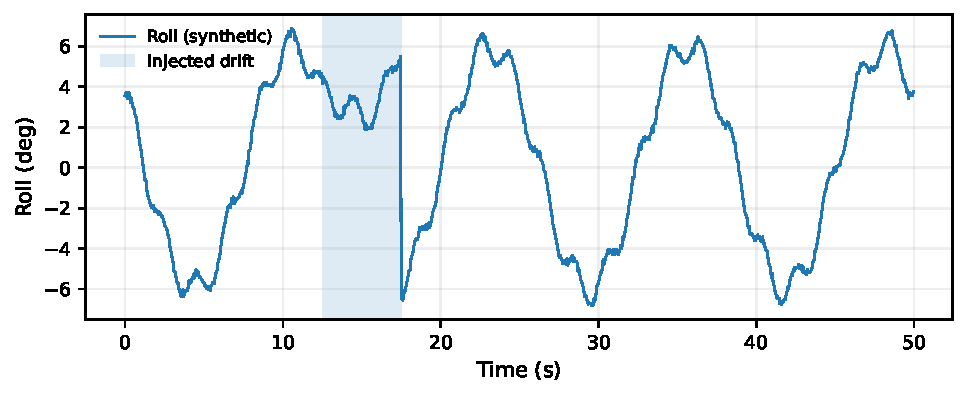
\includegraphics[width=.94\textwidth]{roll-series.pdf}
\gzucaption[合成横滚信号]{第 F10 架次的合成横滚信号与注入漂移区间}
 {Synthetic roll signal and injected drift interval in flight F10}
\label{fig:roll}
\end{figure}

图~\ref{fig:roll} 展示了正常周期项与人为注入的漂移。
图中的横坐标使用秒，异常区间由生成器记录，不由检测结果反推。
这一区分保证真实标签在评估时保持独立。

\section{异常注入规则}
三个测试架次采用相同的区间定义，但基础相位和噪声不同。
所有区间都使用左闭右开的数组约定，见表~\ref{tab:events}。
这种约定与 Python 切片完全一致，避免边界点的重复标记。

\begin{table}[htbp]
\centering
\gzucaption{仅在测试集注入的合成异常}{Synthetic anomalies injected only into test flights}
\label{tab:events}
\begin{tabularx}{\textwidth}{@{}lccX@{}}
\toprule
类型 & 索引区间 & 通道 & 具体操作 \\
\midrule
渐变漂移 & $[250,350)$ & 横滚 & 叠加从 0 到 12 的线性增量 \\
高频振动 & $[520,600)$ & 俯仰 & 叠加幅值 3、频率 5 Hz 的正弦项 \\
恒定偏置 & $[700,780)$ & 电流 & 在基础观测上增加 3 A \\
\bottomrule
\end{tabularx}
\end{table}

正常生成过程没有复杂的传感器饱和、通信丢包、控制回路响应和飞行包线约束。
因此，异常可能比真实故障更规则，也可能与真实机动的统计特征不同。
本文报告这些限制，而不把合成异常描述为经过试飞验证的故障模式。

\section{架次级数据划分}
训练集为 F01--F06，校准集为 F07--F09，测试集为 F10--F12。
表~\ref{tab:split} 给出观测数和有效窗口数。
划分在滑窗前完成，每个架次内部再独立构造窗口。

\begin{table}[htbp]
\centering
\gzucaption{架次级划分与有效窗口数量}{Flight-level splits and valid window counts}
\label{tab:split}
\begin{tabular}{@{}llrrl@{}}
\toprule
子集 & 架次 & 原始点数 & 窗口数 & 用途 \\
\midrule
训练 & F01--F06 & 6000 & \DemoTrainWindows & 标准化与拟合 \\
校准 & F07--F09 & 3000 & \DemoCalWindows & 阈值估计 \\
测试 & F10--F12 & 3000 & \DemoTestWindows & 最终评价 \\
\bottomrule
\end{tabular}
\end{table}

每个架次使用 $L=9$，有效窗口数由命题~\ref{prop:count} 得到。
训练架次的数组可以在统计均值时拼接，但不能在拼接后直接跨边界滑窗。
二者虽然都出现了“拼接”，数学对象却不同：前者计算无序汇总统计，
后者会人为制造本不存在的连续时序上下文。

\section{校准与测试的隔离}
模型超参数和分位数在运行前给定，本例没有利用测试 F1 选择阈值。
改变平滑系数时，重新对校准分数计算阈值，而不是沿用另一组分数尺度的阈值。
测试标签仅在所有分数和阈值确定后进入指标函数。
这条数据依赖关系在算法~\ref{alg:pipeline} 中进一步展开。

为便于复查，原始合成观测保存为 CSV，统计量和配置保存为 JSON，
结果行保存为可直接输入的 LaTeX 片段。正文中的关键统计数字通过宏读取，
重新运行脚本后即可同步更新，避免表格已经变化但摘要仍保留旧数字。
